\definecolor{felt}{RGB}{215,120,30}
\begin{tikzpicture}
\node[anchor=south west,inner sep=0] (img) at (0,0) {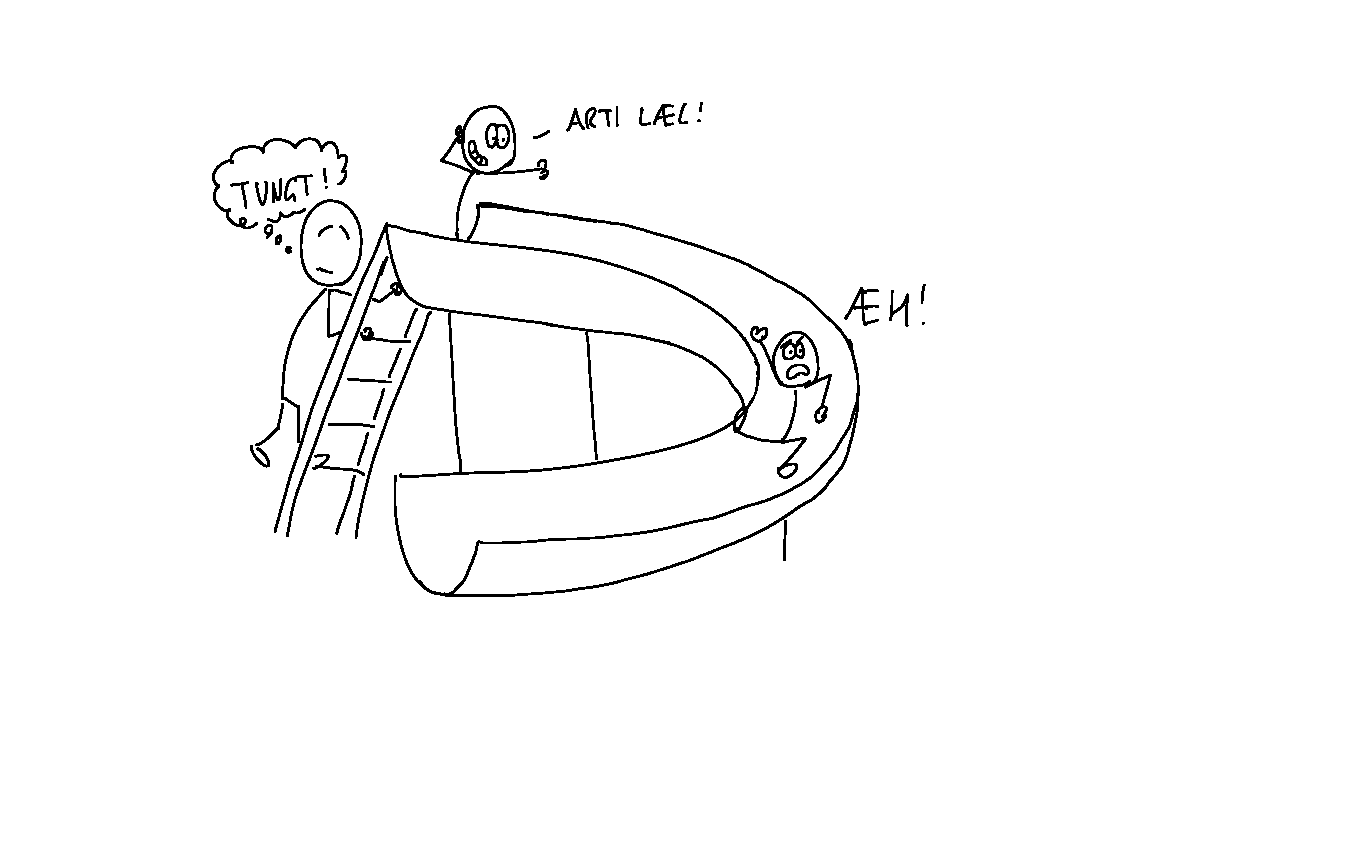
\includegraphics[width=9cm,trim=97 115 202 44,clip]{dashman-stige-sklie.pdf}};
\begin{scope}[x={(img.south east)},y={(img.north west)}]
% nivåene: toppen av stigen og bakken
\draw[dashed,thin] (-0.13,0.729) -- (0.27,0.729);
\draw[dashed,thin] (-0.13,0.138) -- (0.12,0.138);
\draw[<->,very thick,rod] (-0.10,0.138) -- (-0.10,0.729) node[midway,left,align=right,font=\small] {$\Delta E_p = m\mathrm{g}h$\\[1mm] gjort arbeid\\ opp stigen};
% varme fra sklia
\tikzset{varme/.style={->,thick,felt,decorate,decoration={snake,amplitude=.6mm,segment length=2.2mm,post length=1.5mm}}}
\draw[varme] (0.79,0.66) -- ++(0.07,0.09);
\draw[varme] (0.89,0.49) -- ++(0.09,0.03);
\draw[varme] (0.88,0.30) -- ++(0.09,-0.04);
\draw[varme] (0.67,0.12) -- ++(0.06,-0.09);
\draw[varme] (0.42,0.07) -- ++(0.0,-0.10);
\node[felt,font=\small,anchor=west] at (0.98,0.40) {varme};
\node[font=\small,align=center] at (0.62,-0.16) {På vei ned blir hele $\Delta E_p$ brukt opp:\\ den blir til varme i sklia.};
\end{scope}
\end{tikzpicture}
